%%% LISTINGS 

\newsavebox{\IntelSizetIntReduced}
\begin{lrbox}{\IntelSizetIntReduced}
  \hspace{1.5em}
  \begin{lstlisting}
    kernel void A(global double* a) {
      int b = get_global_id(0);
      if (b < -1)
        a[b] = 1;
    }
  \end{lstlisting}
\end{lrbox}

\newsavebox{\OclgrindRaceSwitch}
\begin{lrbox}{\OclgrindRaceSwitch}
  \hspace{1.5em}
  \begin{lstlisting}
  kernel void A(global int* a, global int* b) {
    switch (get_global_id(0)) {
      case 0:
        a[get_global_id(0)] = b[get_global_id(0) + 13];
        break;
      case 2:
        a[get_global_id(0)] = b[get_global_id(0) + 11];
        break;
      case 6:
        a[get_global_id(0)] = b[get_global_id(0) + 128];
    }
    barrier(2);
  }
  \end{lstlisting}
\end{lrbox}

\newsavebox{\AlmostEverythingCrash}
\begin{lrbox}{\AlmostEverythingCrash}
  \hspace{1.5em}
  \begin{lstlisting}
    kernel void A() {
      __builtin_astype(d, uint4);
    }
  \end{lstlisting}
\end{lrbox}

\newsavebox{\OclgrindSemaAssertion}
\begin{lrbox}{\OclgrindSemaAssertion}
  \hspace{1.5em}
  \begin{lstlisting}
    kernel void A(global unsigned char* a, global unsigned char* b) {
      unsigned long c = get_global_id(0);
      d[0] = (mad24(f, (int)(a[0], b[get_global_id(0)])) % (d * (d + 3)) + (c / 2))] * a[c + 1];
    }
  \end{lstlisting}
\end{lrbox}
% This has been forwarded to the LLVM folks https://bugs.llvm.org/show_bug.cgi?id=33897
% __kernel void A(__global float* b) {
%	(float4)(b);
% }

\newsavebox{\IntelPtrCompilerHang}
\begin{lrbox}{\IntelPtrCompilerHang}
  \hspace{1.5em}
  \begin{lstlisting}
    kernel void A(global ulong* a) {
      a[get_global_id(0)] = (ulong)(a + 1);
    }
  \end{lstlisting}
\end{lrbox}
% Another 3± hang:
% kernel void A(global const char* a, global char* b, global char* c) {
%   int d = get_global_id(0);
%   c[d] = get_global_id(0) + c;
% }

% Another 3± hang:
% __kernel void A(global int* a) {
%   local int b[4][3][4][5];
%   b[1][2][3][3] = b[3];
% }

\newsavebox{\NvidiaOptLoopHang}
\begin{lrbox}{\NvidiaOptLoopHang}
  \hspace{1.5em}
  % CLgenProgram.id = 6992
  \begin{lstlisting}
    kernel void A(global float* a, global float* b, global float* c) {
      int d, e, f;
      d = get_local_id(0);
      for (int g = 0; g < 100000; g++)
        barrier(1);
    }
  \end{lstlisting}
\end{lrbox}

\newsavebox{\XeonPhiSpin}
\begin{lrbox}{\XeonPhiSpin}
  \hspace{1.5em}
  \begin{lstlisting}
    kernel void A(global unsigned char* a, unsigned b) {
      a[get_global_id(0)] %= 42;
      barrier(1);
    }
  \end{lstlisting}
\end{lrbox}
% LLVM ERROR: LLVM2PIL: Cannot yet select: 0x7f72a45a7ed0: i8,i8 = umul_lohi 0x7f72a45a87d0, 0x7f72a45a88d0 [ORD=16] [ID=22]
% 0x7f72a45a87d0: i8 = srl 0x7f72a45a7dd0, 0x7f72a42fff90 [ORD=16] [ID=21]
% 0x7f72a45a7dd0: i8,ch = load 0x7f72a41d9438, 0x7f72a4300790, 0x7f72a4300590<LD1[%scevgep2]> [ORD=15] [ID=20]
% 0x7f72a4300790: i64 = add 0x7f72a45a83d0, 0x7f72a45a80d0 [ORD=14] [ID=17]
% 0x7f72a45a83d0: i64,ch = CopyFromReg 0x7f72a41d9438, 0x7f72a45a86d0 [ORD=14] [ID=13]
% 0x7f72a45a86d0: i64 = Register %vreg1 [ID=1]
% 0x7f72a45a80d0: i64,ch = CopyFromReg 0x7f72a41d9438, 0x7f72a45a81d0 [ORD=14] [ID=14]
% 0x7f72a45a81d0: i64 = Register %vreg2 [ID=2]
% 0x7f72a4300590: i64 = undef [ID=3]
% 0x7f72a42fff90: i8 = Constant<1> [ID=9]
% 0x7f72a45a88d0: i8 = Constant<49> [ID=10]

\newsavebox{\IntelOptLoopHang}
\begin{lrbox}{\IntelOptLoopHang}
  \hspace{1.5em}
  \begin{lstlisting}
    kernel void A(global int* a) {
      int b = get_global_id(0);
      while (b < 512) { }
    }
  \end{lstlisting}
\end{lrbox}
% Another example:
%   kernel void A(long a, long b) {
%     while (a > 273444) { }
%   }


\newsavebox{\NvidiaRecursionSegfault}
\begin{lrbox}{\NvidiaRecursionSegfault}
  \hspace{1.5em}
  \begin{lstlisting}
    kernel void A(float4 a, global float4* b, global float4* c, unsigned int d, global double* e, global int2* f, global int4* g, constant int* h, constant int* i) {
      A(a, b, c, d, d, e, f, g, h);
    }
  \end{lstlisting}
\end{lrbox}
% HAND REDUCED:
%
%   kernel void A(constant int2* a, global int* b) { A(b, a); }
\newsavebox{\NvidiaRecursionSegfaultReduced}
\begin{lrbox}{\NvidiaRecursionSegfaultReduced}
  \hspace{1.5em}
  \begin{lstlisting}
    kernel void B(constant int2* a, global int* b) {
      A(b, a);
    }
  \end{lstlisting}
\end{lrbox}

\newsavebox{\BeignetScalarizeInsert}
\begin{lrbox}{\BeignetScalarizeInsert}
  \hspace{1.5em}
  \begin{lstlisting}
    kernel void A(global float4* a) {
      a[get_local_id(0) / 8][get_local_id(0)] = get_local_id(0);
    }
  \end{lstlisting}
\end{lrbox}

\newsavebox{\OclgrindUncorrectedTypos}
\begin{lrbox}{\OclgrindUncorrectedTypos}
  \hspace{1.5em}
  \begin{lstlisting}
    kernel void A(global float* a, global float* b) {
      a[0] = max(a[c], b[2]);
    }
  \end{lstlisting}
\end{lrbox}

\newsavebox{\BeignetPtrIntSpin}
\begin{lrbox}{\BeignetPtrIntSpin}
  \hspace{1.5em}
  \begin{lstlisting}
    kernel void A(global int* a) {
      int b = get_global_id(0);
      a[b] = (6 * 32) + 4 * (32 / 32) + a;
    }
  \end{lstlisting}
\end{lrbox}

\newsavebox{\NvidiaCompileSegfault}
\begin{lrbox}{\NvidiaCompileSegfault}
  \hspace{1.5em}
  \begin{lstlisting}
    kernel void A(global float* a, local float* b, local float* c, int d, int e) {
      int f, g;
      int h = get_local_id(0);
      int i = get_local_id(1);
      int j = get_global_id(0);
      global char* k = c + f * g + f;
      if (f + 1 < h)
        b[f * d + g * h + g] = g * f;
    }
  \end{lstlisting}
\end{lrbox}

\newsavebox{\XeonPhiSegfault}
\begin{lrbox}{\XeonPhiSegfault}
  \hspace{1.5em}
  \begin{lstlisting}
    kernel void A(void) {
      global int* a;
      unsigned int* b;
      b = a[0];
      a[0] = b;
      a[0] = b;
      barrier(1);
      if (get_global_id(0) == 0)
        *a = 0;
      a[get_local_id(0)] = 0;
    }
  \end{lstlisting}
\end{lrbox}

\newsavebox{\IntelVectorizerSegfault}
\begin{lrbox}{\IntelVectorizerSegfault}
  \hspace{1.5em}
  \begin{lstlisting}
    kernel void A() {
      while (true) {
        barrier(1);
      }
    }
  \end{lstlisting}
\end{lrbox}

\newsavebox{\IntelSizetIntUnreduced}
\begin{lrbox}{\IntelSizetIntUnreduced}
  \hspace{1.5em}
  \begin{lstlisting}
    kernel void A(global double* a, global double* b, global double* c, int d, int e) {
      double f;
      int g = get_global_id(0);
      if (g < e - d - 1)
        c[g] = (((e) / d) % 5) % (e + d);
    }
  \end{lstlisting}
\end{lrbox}

\newsavebox{\PoclUndefinedSymbols}
\begin{lrbox}{\PoclUndefinedSymbols}
  \hspace{1.5em}
  \begin{lstlisting}
    kernel void A(local int* a) {
      for (int b = 0; b < 100; b++)
        B(a);
    }
  \end{lstlisting}
\end{lrbox}


\newsavebox{\BeignetCastError}
\begin{lrbox}{\BeignetCastError}
  \hspace{1.5em}
  \begin{lstlisting}
    kernel void A(global float* a, global float* b, global float* c, const int d) {
      int e = get_global_id(0);
      if (e < d)
        c[e] = a[e] + b[e];
      b[e] = (char)(c[e] + d);
    }
  \end{lstlisting}
\end{lrbox}

\newsavebox{\XeonPhiInvalidWrite}
\begin{lrbox}{\XeonPhiInvalidWrite}
  \hspace{1.5em}
  \begin{lstlisting}
    kernel void A(global int* a) {
      a[0] = 1;
      a[-1] = 2;
      a[0] = 3;
    }
  \end{lstlisting}
\end{lrbox}

\newsavebox{\UninitRead}
\begin{lrbox}{\UninitRead}
  \hspace{1.5em}
  \begin{lstlisting}
      kernel void A(global int* a, global int* b) {
        int c[16];
        int d = get_global_id(0);
        a[d] = b[d] + c[d];
      }
  \end{lstlisting}
\end{lrbox}

\newsavebox{\IntelPtrAssertion}
\begin{lrbox}{\IntelPtrAssertion}
  \hspace{1.5em}
  \begin{lstlisting}
    kernel void A(global int* a, global int* b) {
      int c = (int)get_global_id(0);
      a[c] += b;
    }
  \end{lstlisting}
\end{lrbox}

\newsavebox{\IntelScalarAssertion}
\begin{lrbox}{\IntelScalarAssertion}
  \hspace{1.5em}
  \begin{lstlisting}
    kernel void A(global float* a, global float* b, global float* c, local float* d, unsigned int e, unsigned int f) {
      for (unsigned int g = get_local_id(0) + get_local_size(0); g < get_local_size(0); g += get_local_size(0))
        a[2 * get_local_id(0) + 1] = get_local_id(0);
    }
  \end{lstlisting}
\end{lrbox}

\newsavebox{\BeignetTernary}
\begin{lrbox}{\BeignetTernary}
  \hspace{1.5em}
  \begin{lstlisting}
    kernel void A(global int* a, global int* b, global int* c) {
      c[0] = (a[0] > b[0]) ? a[0] : 0;
      c[2] = (a[3] <= b[3]) ? a[4] : b[5];
      c[4] = (a[4] <= b[5]) ? a[7] : b[7];
      c[7] = (a[7] < b[0]) ? a[0] : (a[0] > b[1]);
    }
  \end{lstlisting}
\end{lrbox}
% HAND REDUCED:
%
%   kernel void A(global int* a, global int* b, global int* c) {
%     c[0] = 100;
%     c[1] = (a[3] <= b[4]) ? a[4] : b[5];
%   }

\newsavebox{\BeignetTernarySmaller}
\begin{lrbox}{\BeignetTernarySmaller}
  \hspace{1.5em}
  \begin{lstlisting}
    kernel void A(global int* a, global int* b, global int* c) {
      c[0] = (a[0] > 0) ? a[0] : b[1];
      c[1] = (a[1] <= b[1]) ? a[0] : b[0];
    }
  \end{lstlisting}
\end{lrbox}

\newsavebox{\IntelGtDoubleAssertion}
\begin{lrbox}{\IntelGtDoubleAssertion}
  \hspace{1.5em}
  \begin{lstlisting}
    kernel void A(read_only image2d_t a, global double2* b) {
      b[0] = get_global_id(0);
    }
  \end{lstlisting}
\end{lrbox}

\newsavebox{\IntelDeclDoesntDeclareAnything}
\begin{lrbox}{\IntelDeclDoesntDeclareAnything}
  \hspace{1.5em}
  \begin{lstlisting}
    kernel void A() {
      char a;
      int b;
      int const;
    }
  \end{lstlisting}
\end{lrbox}

\newsavebox{\AddressQualifiedAutoVar}
\begin{lrbox}{\AddressQualifiedAutoVar}
  \hspace{1.5em}
  \begin{lstlisting}
    kernel void A(global float4* a, global float4* b, global float4* c, global float4* d, global float4* e, float f) {
      unsigned int g = get_global_id(0);
      int h = get_global_size(0);
      constant sampler_t i = 0x0000 | 0x0004 | 0x0000;
      unsigned int j = g * (1 << ((h % 4) - (2)));
    }
  \end{lstlisting}
\end{lrbox}

\newsavebox{\NvidiaLocalGlobalSegfault}
\begin{lrbox}{\NvidiaLocalGlobalSegfault}
  \hspace{1.5em}
  \begin{lstlisting}
    kernel void A(global int* a) {
      local int b[2][3][4][5];
      if (get_global_id(0) == 0)
        a = b[0];
    }
  \end{lstlisting}
\end{lrbox}

\newsavebox{\NvidiaLocalSegfault}
\begin{lrbox}{\NvidiaLocalSegfault}
  \hspace{1.5em}
  \begin{lstlisting}
    kernel void A(global uchar4* a, const int b) {
      local int c[16];
      local float8* d = a + 133;
      atomic_cmpxchg(c, 10, 13);
    }
  \end{lstlisting}
\end{lrbox}


% Program ID: 35612
\newsavebox{\IntelPostDominanceFrontier}
\begin{lrbox}{\IntelPostDominanceFrontier}
  \hspace{1.5em}
  \begin{lstlisting}
    kernel void A() {
      while (true)
        barrier(1);
    }
  \end{lstlisting}
\end{lrbox}
% Another:
% kernel void A(local int* a) {
%   while (1) {
%   }
% }
%
% And another:
%    kernel void A(global int* a) {
%      bool b;
%      int c;
%      for (b = 0; b < 100; b++)
%        a[c] += a[c];
%    }
%
% One more:
%   kernel void A(global int* a, global int* b) {
%     int c = get_global_id(0);
%     int d = 0;
%     while (d < 1024)
%       a[c] = d;
%   }

\newsavebox{\IntelPredicator}
\begin{lrbox}{\IntelPredicator}
  \hspace{1.5em}
  \begin{lstlisting}
    kernel void A(global int* a) {
      int b = get_global_id(0);
      while (b < *a)
        if (a[0] < 0)
          a[1] = b / b * get_local_id(0);
    }
  \end{lstlisting}
\end{lrbox}

\newsavebox{\IntelPrepareKernelArgs}
\begin{lrbox}{\IntelPrepareKernelArgs}
  \hspace{1.5em}
  \begin{lstlisting}
    kernel void A(int a, global int* b) {
      int c = get_global_id(0);
      int d = work_group_scan_inclusive_max(c);
      b[c] = c;
    }
  \end{lstlisting}
\end{lrbox}

\newsavebox{\IntelDAGInstrSelection}
\begin{lrbox}{\IntelDAGInstrSelection}
  \hspace{1.5em}
  \begin{lstlisting}
    kernel void A(global half* a, global int* b, global bool* c, int d, int e) {
      int f = get_global_id(0);
      int g = get_global_id(1) * e;
      if (f < e)
        a[f] = b[f];
    }
  \end{lstlisting}
\end{lrbox}

\newsavebox{\IntelSPIRMetadata}
\begin{lrbox}{\IntelSPIRMetadata}
  \hspace{1.5em}
  \begin{lstlisting}
    kernel void A() {
      local float a;
      A(a);
    }
  \end{lstlisting}
\end{lrbox}

\newsavebox{\IntelRemoveDupeBarrier}
\begin{lrbox}{\IntelRemoveDupeBarrier}
  \hspace{1.5em}
  \begin{lstlisting}
    kernel void A() {
      local int a[10];
      local int b[16][16];
      a[1024 + (2 * get_local_id(1) + get_local_id(0)) + get_local_id(0)] = 6;
      barrier(b);
    }
  \end{lstlisting}
\end{lrbox}

\newsavebox{\IntelCombineRedundant}
\begin{lrbox}{\IntelCombineRedundant}
  \hspace{1.5em}
  \begin{lstlisting}
    kernel void A(global float* a, global float* b, global float* c, const int d) {
      for (unsigned int e = get_global_id(0); e < d; e += get_global_size(0))
        for (unsigned f = 0; f < d; ++f)
          e += a[f];
    }
  \end{lstlisting}
\end{lrbox}


\section{Evaluation}%
\label{sec:eval}

We report on the results of extensive DeepSmith testing of the 10 OpenCL testbeds from Table~\ref{tab:platforms} over four months. We found bugs in all the compilers we tested --- every compiler crashed, and every compiler generated programs which either crash or silently compute the wrong result. To date, we have submitted XX bug reports to compiler vendors. We first provide examples of compile-time defects found, including an analysis on front-end stability of every LLVM release in the past 2 years. We follow this with examples of runtime defects. Finally, we compare our approach to the state-of-the-art in OpenCL compiler fuzzing.

Unless stated otherwise, all code listings are presented verbatim as generated by DeepSmith --- only uneeded whitespace and braces have been removed to save space.

\subsection{Compile-time Defects}%
\label{subsec:compile-time-defects}

We found numerous cases where kernels trigger a crash in the compiler (and as a result, the host process), or the compiler to loop indefinitely.

DeepSmith is highly effective at crashing compilers. We believe that our approach contributes a significant improvement for generating plausibly-erroneous code over prior random-enumeration approaches.

% \texttt{kernel void A(global float* a) { (float4)(a); }}

\begin{figure}
  \centering %
  \subfloat[Testbeds $1\pm$, $2\pm$ segementation fault due to implicit address space conversion.]{%
    \noindent\mbox{\parbox{\columnwidth}{\usebox{\NvidiaRecursionSegfault}}}%
    \label{lst:nvidia-recursion-segfault}
  }\\%
%  \subfloat[Reduced version of Figure~\ref{lst:nvidia-recursion-segfault}.]{%
%    \noindent\mbox{\parbox{\columnwidth}{\usebox{\NvidiaRecursionSegfaultReduced}}}%
%    \label{lst:nvidia-recursion-segfault}
%  }\\%
%  \subfloat[Testbed $10\pm$ assertion \emph{Uncorrected typos!} during semantic analysis.]{%
%    \noindent\mbox{\parbox{\columnwidth}{\usebox{\OclgrindSemaAssertion}}}%
%    \label{lst:oclgrind-uncorrected-typos}
%  }\\%
  \subfloat[Testbed $10\pm$ assertion \emph{Uncorrected typos!} during semantic analysis.]{%
    \noindent\mbox{\parbox{\columnwidth}{\usebox{\OclgrindUncorrectedTypos}}}%
    \label{lst:oclgrind-uncorrected-typos}
  }\\%
  \subfloat[Of the 10 compilers we tested, 6 crash with segfault when compiling this kernel.]{%
    \noindent\mbox{\parbox{\columnwidth}{\usebox{\AlmostEverythingCrash}}}%
    \label{lst:almost-everything-crash}
  }\\%
  \subfloat[Testbeds $3\pm$ assertion \emph{sel.hasDoubleType()} during code generation.]{%
    \noindent\mbox{\parbox{\columnwidth}{\usebox{\IntelGtDoubleAssertion}}}%
    \label{lst:intel-gt2-double-assertion}
  }\\%
  \subfloat[Testbeds $3\pm$ assertion \emph{scalarizeInsert} during code generation.]{%
    \noindent\mbox{\parbox{\columnwidth}{\usebox{\BeignetScalarizeInsert}}}%
    \label{lst:beignet-scalarize-insert}
  }\\%
%  \subfloat[Testbeds $7\pm$ segmentation fault.]{%
%    \noindent\mbox{\parbox{\columnwidth}{\usebox{\XeonPhiSegfault}}}%
%    \label{lst:xeon-phi-segfault}
%  }\\%
  \caption{Example kernels which crash compilers.}%
\end{figure}
 
\paragraph{Semantic Analysis Failures} %
We discovered many compiler crashes which can be attributed to improper or missing error handling. Testing compilers under invalid inputs is important.

Figure~\ref{lst:nvidia-recursion-segfault} induces an error in NVIDIA compilers due to an implicit global to constant address qualifiers.

Undeclared identifiers should be an easy error; yet, the undeclared identifier \texttt{c} in Figure~\ref{lst:oclgrind-uncorrected-typos} raises an assertions in the compiler frontend during semantic analysis of the AST of testbed $10\pm$.

\paragraph{Compiler-specific code} %
Since the expressiveness of our approach is bounded only by the handwritten programs we train on, DeepSmith will occasionally emit compiler-specific code, such as invoking compiler builtins. Figure~\ref{lst:almost-everything-crash} crashes 6 of the 10 compilers we tested crashed with segmentation faults.

\paragraph{Code generation} %
Figures~\ref{lst:intel-gt2-double-assertion} and~\ref{lst:beignet-scalarize-insert} cause failures in the LLVM code generator backend.

% CLgen result ID 994
TODO: Testbed $3\pm$ assertion in \emph{gbe::GenEncoder::handleDouble}

\paragraph{Parser Failures} %
Parser development is a mature and well understood practise. To our surprise, we uncovered parser errors. For example, the following three code samples induce crash errors during parsing of compound statements in both Testbeds $5\pm$ and $7\pm$:

\begin{enumerate}
% Hand reduction of a 40 line kernel:
\item \texttt{void A() \{ (global a*)()}
% Hand reduction of a 52 line kernel:
\item \texttt{void A() \{ void* a; uint4 b = 0; b = (b > b) ? a : a}
% 68 line kernel:
\item \texttt{void A() \{ double2 k; return (float4)(k, k, k, k)}
\end{enumerate}

Each code fragment was hand-reduced from a 40, 52, and 68 DeepSmith sample, respectively. It took about 10 minutes to perform all three reductions by hand, producing these minimal code samples which we have reported. In total, we have generated \cc{XXX} programs which crash parsers.


\begin{figure}
  \centering
  % Result id: 110876
  \subfloat[\emph{Post-Dominance Frontier Construction} pass.]{%
    \noindent\mbox{\parbox{\columnwidth}{\usebox{\IntelPostDominanceFrontier}}}%
    \label{lst:intel-postdominance-frontier}
  }\\%
  % Program id: 31656
  \subfloat[\emph{Predicator} pass.]{%
    \noindent\mbox{\parbox{\columnwidth}{\usebox{\IntelPredicator}}}%
    \label{lst:intel-predicator}
  }\\%
  \subfloat[\emph{Combine redundant instructions} pass.]{%
    \noindent\mbox{\parbox{\columnwidth}{\usebox{\IntelCombineRedundant}}}%
    \label{lst:intel-spir-metadata}
  }\\%
  % Program id: 10596
  \subfloat[\emph{PrepareKernelArgs} pass.]{%
    \noindent\mbox{\parbox{\columnwidth}{\usebox{\IntelPrepareKernelArgs}}}%
    \label{lst:intel-prepare-kernel-args}
  }\\%
  % Program id: 37443
  \subfloat[\emph{Add SPIR related module scope metadata} pass.]{%
    \noindent\mbox{\parbox{\columnwidth}{\usebox{\IntelSPIRMetadata}}}%
    \label{lst:intel-spir-metadata}
  }\\%
  % Program id: 44105
  \subfloat[\emph{Intel OpenCL RemoveDuplicationBarrier} pass.]{%
    \noindent\mbox{\parbox{\columnwidth}{\usebox{\IntelRemoveDupeBarrier}}}%
    \label{lst:intel-spir-metadata}
  }\\%
  % CLgen result ID 452598
  % \cc{TODO: Intel pass \emph{X86 DAG->DAG Instruction Selection}}
  % kernel void A(global half* a) {
  %   int b = get_global_id(0);
  %   a[b] = b * b;
  % }
  % CLgen result ID 1903475
  % \cc{TODO: Intel pass \emph{Intel OpenCL Barrier}}
  % kernel void A(global float* a, global float* b, const int c) {
  %   int d = get_global_id(8);
  %   b[d] = a[d] + b[d];
  % }
  \caption{Example kernels which crash Intel compiler passes.}%
  \label{lst:intel-passes}
\end{figure}

\paragraph{Intel Pass Failures} %
Intel compilers will ocassionally emit a stack trace upon crashing, identifying the failure point in a specific pass. To date, we have triggered crashes in 10 different Intel passes. Figure~\ref{lst:intel-passes} provides examples.


\begin{figure}
  \centering %
  \subfloat[]{%
    \noindent\mbox{\parbox{\columnwidth}{\usebox{\NvidiaLocalGlobalSegfault}}}%
    \label{lst:nvidia-local-global-sefault}
  }\\%
  \subfloat[]{%
      \noindent\mbox{\parbox{\columnwidth}{\usebox{\NvidiaLocalSegfault}}}%
      \label{lst:nvidia-local-global-sefault}
    }\\%
  \caption{Kernels containing pointer assignments which segfault Nvidia compilers.}%
  \label{lst:nvidia-silent-segfaults}
\end{figure}

\paragraph{Nvidia silent segfaults} %

Of the compilers we tested, Nvidia's are the least verbose. This makes identifying root causes more difficult. Figure~\ref{lst:nvidia-silent-segfaults} shows examples of crashes we identified as caused by pointer assignments. Without error messages and source code, we can only report a couple of errors and move on.


\begin{figure}
  \centering %
  \subfloat[Testbed $1+$ hangs during optimization of kernels with large loop bounds. Testbeds $1-$ and $2\pm$ compile in under 1 second.]{%
    \noindent\mbox{\parbox{\columnwidth}{\usebox{\NvidiaOptLoopHang}}}%
    \label{lst:nvidia-opt-loop-hang}
  }\\%
  \subfloat[Testbeds $4+$, $5+$, $6+$, $7+$ hang during optimization of kernels with non-terminating loops.]{%
    \noindent\mbox{\parbox{\columnwidth}{\usebox{\IntelOptLoopHang}}}%
    \label{lst:intel-inf-loop}
  }\\%
  \subfloat[Testbeds $7\pm$ loops indefinitely, consuming 100\% CPU usage.]{%
    \noindent\mbox{\parbox{\columnwidth}{\usebox{\XeonPhiSpin}}}%
    \label{lst:xeon-phi-spin}
  }\\%
  \subfloat[Testbed $3\pm$ loop indefinitely, leaking memory until the entire system memory is depleted and the process crashes.]{%
    \noindent\mbox{\parbox{\columnwidth}{\usebox{\BeignetPtrIntSpin}}}%
    \label{lst:beignet-ptr-int-spin}
  }\\%
% Testbed 3± ptr-int spin:
%  \subfloat[]{%
%    \noindent\mbox{\parbox{\columnwidth}{\usebox{\IntelPtrCompilerHang}}}%
%    \label{lst:gt2-compiler-hang}
%  }\\%
  \caption{Example kernels which hang compilers.}%
  \label{lst:compiler-hangs}%
\end{figure}


\paragraph{Compiler Hangs} %
Some compiler crashes are optimization sensitive. Testbeds $1+$ and $2+$ hang on large loop bounds, shown in Figure~\ref{lst:nvidia-opt-loop-hang} \cc{how large does the loop bound have to be?}.

Figure~\ref{lst:intel-inf-loop} All commericial Intel compilers we tested hang during optimization of non-terminating loops.

Figure~\ref{lst:xeon-phi-spin} --- bizarrely, Testbed $7\pm$ loops indefinitely during compilation of this simple kernel.

Testbed $3\pm$ loops indefinitely while assigning a value from a pointer address Figure~\ref{lst:beignet-ptr-int-spin}. While spinning, the compiler consumes 100\% CPU and leaks memory.


\paragraph{Unreachable code} %
To date we have identified 207 distinct cases which trigger unreachable code failures. \cc{How many *distinct* traces?}


\paragraph{Silent crashes} %
110 distinct test cases which crash testbed $9\pm$ during compilation, all silently.


%\begin{figure}
%  \centering %
%  \subfloat[Testbeds $1\pm$, $2\pm$, $3\pm$ reject address space-qualified automatic variables.]{%
%    \noindent\mbox{\parbox{\columnwidth}{\usebox{\AddressQualifiedAutoVar}}}%
%    \label{lst:adress-qualified-autovar}
%  }\\%  
%  \subfloat[Testbeds $4\pm$, $6\pm$ reject anonymous declarations. %\emph{declaration doesn't declare anything}.
%    % All other testbeds compile, some with a warning.
%    ]{%
%    \noindent\mbox{\parbox{\columnwidth}{\usebox{\IntelDeclDoesntDeclareAnything}}}%
%    \label{lst:intel-decl-doesnt-declare-anything}
%  }\\%
%  \caption{Well-formed kernels which do not compile.}%
%\end{figure}

\paragraph{Build Failures} %
Some compilers are more permissive then others.

%Figure~\ref{lst:intel-decl-doesnt-declare-anything}
Empty declarations (e.g. \texttt{int;}) are rejected by some Intel compilers.

Testbeds~$4\pm$, $6\pm$, $9\pm$ reject out-of-range literal values e.g. \texttt{int i = 0xFFFFFFFFFFFFFFFFFFFFFFFF}, whilst testbeds $3\pm$, $5\pm$, $7\pm$, $8\pm$, and $10\pm$ interpret the literal as an \texttt{unsigned long long} and implicitly cast to an integer value (-1); testbeds $1\pm$, $2\pm$ omit no warning.

Testbeds $1\pm$, $2\pm$, $3\pm$ rejects address space qualifiers on automatic variables.

% T3± mad24() result ID: 891687
On Testbed~$3\pm$, the statment \texttt{int n = mad24(a, (32), get\_global\_size(0));} is rejected as ambiguous.


\begin{figure}
  \centering %
  \includegraphics[width=.95\columnwidth]{build/img/clang-crashes}%
  \caption{%
    Crash rate of every LLVM release in the past 24 months compiling 75k DeepSmith kernels using Clang front-end.% 2 years of development has lead to a tenfold decrease in crash rate.
  }%
  \label{fig:clangs} %
\end{figure}

\begin{table}
  \scriptsize %
  \centering %
  \begin{tabular}{r|ccccccc}
\toprule
{} &   3.6.2 &   3.7.1 &   3.8.1 &   3.9.1 &   4.0.1 &   5.0.0 &   6.0.0 \\
\midrule
A1 &  \xmark &  \xmark &  \xmark &  \xmark &  \xmark &  \xmark &  \xmark \\
A2 &         &  \xmark &  \xmark &         &         &         &         \\
A3 &         &         &         &         &         &         &  \xmark \\
A4 &         &         &         &         &         &         &  \xmark \\
A5 &  \xmark &         &         &         &         &         &         \\
A6 &  \xmark &         &         &         &         &         &         \\
A7 &         &         &         &  \xmark &  \xmark &         &         \\
\bottomrule
\end{tabular}

  \caption{%
    Distinct Clang front-end assertions triggered by DeepSmith, and the number of distinct unreachables.%
  }
  \label{tab:clangs}
\end{table}


\paragraph{Comparison of Clang Front-ends}%
% \label{subsec:clangs}

Many compilers use a common Clang front-end. Perhaps that's why Figure~\ref{lst:almost-everything-crash} fails on so many testbeds.

Using debug + assert builds over every LLVM release in the past 24 months, compile 75,000 DeepSmith kernels using clang frontend (no code generation, just lexer, parser, and typechecker).

Figure~\ref{fig:clangs} shows the crash rate of Clang front-ends. Progress is good. There's a tenfold decrease in crash rate in 2 years. 

Table~\ref{tab:clangs} shows whether each of 7 distinct assertions were raised. Assertion 1 (uncorrected typos) is raised on all compiler versions --- see Figure~\ref{lst:oclgrind-uncorrected-typos} for an example.

TODO: Report the 5 distinct crashes in LLVM trunk.

TODO: What programs crash all versions? What programs are regressions?


\subsection{Runtime Defects}

\begin{figure}
  \centering %
  \subfloat[Testbeds $4+$, $6+$ incorrectly optimize the \texttt{if} statement, causing the conditional branch to execute (it shouldn't). This pattern of integer comparison to thread ID is widely used.]{%
    \noindent\mbox{\parbox{\columnwidth}{\usebox{\IntelSizetIntUnreduced}}}%
    \label{lst:intel-size_t-int-unreduced}
  }\\%
  \subfloat[A race condition in \texttt{switch} statement evaluation causes $10\pm$ to sporadically crash when executed with a global size $> 1$.]{%
    \noindent\mbox{\parbox{\columnwidth}{\usebox{\OclgrindRaceSwitch}}}%
    \label{lst:oclgrind-race-switch}
  }\\%
  \subfloat[Testbed $3\pm$ silently miscompiles ternary ops in which the operands are global buffers \cc{double check the cause}.]{%
    \noindent\mbox{\parbox{\columnwidth}{\usebox{\BeignetTernary}}}%
    \label{lst:pocl-undefined-symbols}
  }\\%
  \subfloat[Compilation should fail due to call to undefined function \texttt{B()}; Testbeds $6\pm$ silently succeed then crash upon kernel execution.]{%
    \noindent\mbox{\parbox{\columnwidth}{\usebox{\PoclUndefinedSymbols}}}%
    \label{lst:pocl-undefined-symbols}
  }\\%
%  \subfloat[Testbeds $3\pm$ incorrect cast yields \texttt{b[e] = 127}, not \texttt{b[e] = 0}. \cc{TODO: Is char overflow defined?}]{%
%    \noindent\mbox{\parbox{\columnwidth}{\usebox{\BeignetCastError}}}%
%    \label{lst:beignet-cast-error}
%  }\\%
  \caption{Example kernels which are miscompiled.}%
\end{figure}


Extensive prior work by EMI/CSmith/SPE extensively stress-test middle-end to uncover miscompilations. Grammar based enumeration is highly effective at this task, yet is bounded by the expressiveness of the grammar. Here we provide examples of bugs which cannot currently be discovered by the state-of-the-art grammar approach.

\paragraph{Thread-dependent Flow Control} CLSmith does not support this (because of the risk of barrier divergence).

A common pattern in OpenCL is to obtain the thread identity, often as an \texttt{int}, and to compare this against some fixed value to determine whether or not to complete a unit of work. DeepSmith, having modeled the frequency with which this pattern occurs in real handwritten code, generates many programs containing permutations of this pattern. And in doing so, exposed an error in the optimizer of two Testbeds $4+$, $6+$ which causes the \texttt{if} statement of Figure~\ref{lst:intel-size_t-int-unreduced} to be executed when the kernel is compiled with optimizations enabled.
%
% cd ~/data/kernels/github-pp
% ls | xargs egrep -l 'int [A-Z]+ = get_global_id\(' -- | wc -l
% >> 2144
% ls | wc -l
% >> 4655
\cc{Too strongly worded:} This is troubling --- 46\% of OpenCL kernels on GitHub use this ($tid \rightarrow$ int, \texttt{if (tid < \ldots) \{\ldots\}}) pattern to guard against invalid memory accesses. \cc{TODO: a common pattern is ... We found 46\% of ... we found that this permutation (see listing) is miscompiled}. CLSmith does not support conditional control flow based on thread ID. % CLSmith prevents thread identity from influencing control flow in order to prevent barrier divergence.

Figure~\ref{lst:oclgrind-race-switch} shows a simple program in which thread identity determines the program output. We found that this test case would sporadically crash Testbeds~$10\pm$, an OpenCL device simulator and debugger. Upon reporting to the developers, the underlying cause was quickly diagnosed as a race condition in \texttt{switch} statement evaluation, and fixed within a week.

\paragraph{Device Memory} CLSmith kernels do not accept inputs. All data is allocated statically in global structs.

Figure~\ref{lst:pocl-undefined-symbols} exposed a bug in Testbed $3\pm$ in which ternary operations do not execute if their operands are global buffers (i.e. device allocated memory).

\cc{TODO: double check that the global buffers are the culprit. Can CLSmith produce anything close?}

\paragraph{Latent Compilation Errors} Sometimes, invalid inputs may go undetected. Since CLSmith enumerates well-defined programs, this class of bugs cannot be discovered.

Figure~\ref{lst:pocl-undefined-symbols} exposes a bug in which a kernel containing an undefined symbol will successfully compile without warning, then crash the program when attempting to run the kernel. \cc{TODO: CLSmith does not catch this class of bugs (undefined symbols}.

% \paragraph{Type conversion} Figure~\ref{lst:beignet-cast-error}. The code performs int and float addition, casting the result to a char, then storing in float. Changing any one of those makes the problem go away.


%\subsection{Gray Areas and False Positives}
%
%\cc{DELETE ME}
%
%Some compilers are more permissive than others - some compilers will reject kernels with out-of-range literals \emph{integer literal is too large}.
%
%None of the three statements in Figure~\ref{lst:xeon-phi-invalid-write} are executed by testbeds~$7\pm$, all other configurations return the final value. In testbeds $1\pm$ (but not $2\pm$), out-of-bounds memory reads and writes can be used to overflow into neighboring kernel arguments. In both cases, oclgrind can automatically catch the inalid accesses to prevent false-positives, but perhaps should results may be interesting for testing robustness / security. E.g.~\cite{Holler2012}.
%
%
%
%\begin{figure}
%  \centering %
%  \subfloat[The out-of-range write on line 3 is invalid, but does not affect execution of lines 2 and 4 for all testbeds except $7\pm$. On Testbeds $7\pm$, lines 2 and 4 execute when the invalid write has an index $1 \le i < 44032$, and not  when index $i \ge 44032$ or $i < 0$.]{%
%    \noindent\mbox{\parbox{\columnwidth}{\usebox{\XeonPhiInvalidWrite}}}%
%    \label{lst:xeon-phi-invalid-write}
%  }\\%
%  \caption{Example kernels which mis-match.}%
%  \label{lst:gray-areas}%
%\end{figure}
%
%\begin{figure}
%  \centering %
%  \subfloat[Read of uninitialized automatic variable \texttt{c}.]{%
%    \noindent\mbox{\parbox{\columnwidth}{\usebox{\UninitRead}}}%
%    \label{lst:uninit-read}
%  }\\%
%  \caption{False positives.}%
%  \label{lst:uninit-read}%
%\end{figure}


\subsection{Comparison to State-of-the-art}%
\label{subsec:vs_clsmith}

In this section we compare DeepSmith to CLSmith~\cite{Lidbury2015a}, the state-of-the-art in OpenCL compiler testing.

\paragraph{Experimental Setup}

We ran each program generator using its default configuration for 48 hours on each of the 10 testbeds of Table~\ref{tab:platforms}. We ran the tests twice, first with optimizations disabled ($-$), then with optimizations enabled ($+$). Total runtime for a test case consists of the generation time, and the time to execute the test case.


\paragraph{Results Overview}

\begin{table*}
  \scriptsize %
  \centering %
  \begin{tabular}{lll | rrrrr | rrrrr }
  \toprule
  & & & \multicolumn{5}{c|}{\textbf{CLSmith}} & \multicolumn{5}{c}{\textbf{CLgen}} \\
  \textbf{\#.} & \textbf{Device} & $\pm$ &
  \textbf{w} & \textbf{bf} & \textbf{c} & \textbf{to} & \textbf{\% of total} &
  \textbf{w} & \textbf{bf} & \textbf{c} & \textbf{to} & \textbf{\% of total} \\
  \midrule
  \multirow{ 2}{*}{1} & \multirow{ 2}{*}{GeForce GTX 1080} & $-$ & 0 & 0 & 17 & 25 & 0.8\%       & 10 & 45 & 28 & 5 & 0.4\% \\& & $+$ & 5 & 0 & 63 & 15 & 1.5\% & 14 & 28 & 12 & 14 & 0.3\% \\
\hline
\multirow{ 2}{*}{2} & \multirow{ 2}{*}{GeForce GTX 780} & $-$ & 3 & 0 & 22 & 37 & 0.9\%       & 617 & 406 & 65 & 42 & 25.9\% \\& & $+$ & 0 & 0 & 10 & 37 & 0.7\% & 281 & 375 & 37 & 68 & 22.9\% \\
\hline
\multirow{ 2}{*}{3} & \multirow{ 2}{*}{Intel HD Haswell GT2} & $-$ & 0 & 0 & 0 & 0 & 0.0\%       & 108 & 473 & 20 & 0 & 1.2\% \\& & $+$ & 0 & 0 & 0 & 0 & 0.0\% & 22 & 39 & 6 & 0 & 0.2\% \\
\hline
\multirow{ 2}{*}{4} & \multirow{ 2}{*}{Intel E5-2620 v4} & $-$ & 0 & 563 & 192 & 0 & 11.2\%       & 3 & 10 & 93 & 1 & 0.3\% \\& & $+$ & 0 & 595 & 434 & 1 & 14.5\% & 1 & 7 & 110 & 3 & 0.3\% \\
\hline
\multirow{ 2}{*}{5} & \multirow{ 2}{*}{Intel E5-2650 v2} & $-$ & 0 & 0 & 0 & 0 & 0.0\%       & 2 & 65 & 131 & 1 & 23.9\% \\& & $+$ & 0 & 0 & 61 & 0 & 1.1\% & 8 & 66 & 138 & 3 & 25.1\% \\
\hline
\multirow{ 2}{*}{6} & \multirow{ 2}{*}{Intel i5-4570} & $-$ & 0 & 570 & 0 & 0 & 8.3\%       & 15 & 362 & 156 & 10 & 20.2\% \\& & $+$ & 0 & 629 & 0 & 0 & 8.2\% & 6 & 167 & 170 & 10 & 31.6\% \\
\hline
\multirow{ 2}{*}{7} & \multirow{ 2}{*}{Intel Xeon Phi} & $-$ & 6 & 0 & 131 & 5 & 2.8\%       & 19 & 30 & 0 & 73 & 0.9\% \\& & $+$ & 1 & 0 & 0 & 4 & 0.3\% & 12 & 32 & 0 & 65 & 0.8\% \\
\hline
\multirow{ 2}{*}{8} & \multirow{ 2}{*}{POCL (Intel E5-2620)} & $-$ & 0 & 0 & 56 & 2 & 0.9\%       & 2 & 6 & 850 & 7 & 2.8\% \\& & $+$ & 0 & 0 & 8 & 18 & 0.4\% & 1 & 7 & 930 & 1 & 2.9\% \\
\hline
\multirow{ 2}{*}{9} & \multirow{ 2}{*}{ComputeAorta (Intel E5-2620)} & $-$ & 0 & 0 & 0 & 11 & 0.2\%       & 15 & 620 & 85 & 0 & 38.8\% \\& & $+$ & 9 & 0 & 177 & 35 & 3.1\% & 19 & 563 & 49 & 6 & 39.4\% \\
\hline
\multirow{ 2}{*}{10} & \multirow{ 2}{*}{Oclgrind Simulator} & $-$ & 0 & 0 & 0 & 8 & 0.4\%       & 6 & 3 & 13 & 80 & 0.3\% \\& & $+$ & 0 & 0 & 0 & 14 & 0.7\% & 7 & 2 & 9 & 50 & 0.2\% \\
  \bottomrule
\end{tabular}


  \caption{%
    % CLSmith total ``interesting'': 19415
    % DeepSmith total ``interesting'': 8272
    Results from 48 hours of testing using CLSmith and DeepSmith. Testbed \#. as per Table~\ref{tab:platforms}. $\pm$ denotes optimizations off ($-$) vs on ($+$). The remaining columns denote the number of build crash (\textbf{bc}), build timeout (\textbf{bto}), build failure (\textbf{bf}), runtime crash (\textbf{c}), timeout (\textbf{to}), and pass (\textbf{\cmark}) results. \cc{remove ``Total'' row for submission}%
  }
  \label{tab:megatable}
\end{table*}

\begin{figure}
  \centering %
  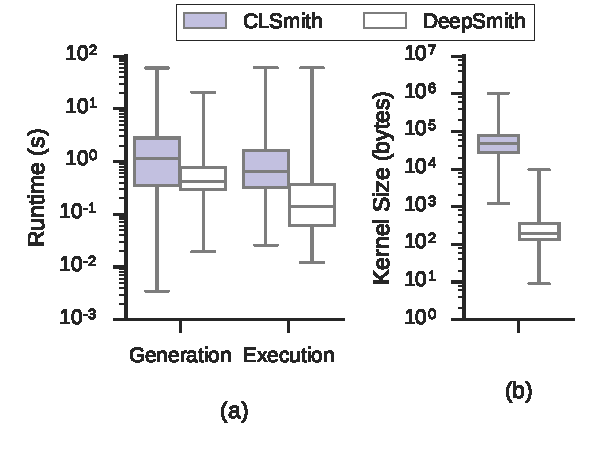
\includegraphics[width=\columnwidth]{build/img/vs-clsmith}%
  \vspace{-1em}
  \caption{%
    Comparison of runtimes and test case sizes. DeepSmith test cases are on average evaluated $3.03\times$ faster than CLSmith ($2.45\times$, and $4.46\times$ for generation and execution, respectively), and are two orders of magnitude smaller.
    % Runtimes, excluding timeouts. .%
%    Total speedup is 3.03x
%    CLgen generation is 2.45x faster than CLSmith
%    CLgen execution is 4.46x faster than CLSmith
%    CLgen reduction is 66.54x faster than CLSmith
  }%
  \label{fig:vs-clsmith} %
\end{figure}

Table~\ref{tab:megatable} shows the results of 48 hours of consecutive testing for each of the platforms from Table~\ref{tab:platforms}.

% Total CLSmith test cases ran: 285077
% Total DeepSmith test cases ran: 1821311
Each testbed evaluated an average of 29k CLSmith and 182k DeepSmith test cases, with an average time per test case of 12.1s and 1.90s respectively. The sixfold increase in testing throughput achieved by DeepSmith is a result of XXX. Figure~\ref{fig:vs-clsmith}a shows the times taken to generate and execute test cases, excluding timeouts. DeepSmith generation time is proportional to program length. For Clsmith, generation time depends on the number of rejections which are required before production of statically verified code is correct \cc{\ldots}.

Optimization level generally does not affect testing throughput significantly, with the exception of testbed $7+$, in which the slow compilation of kernels containing structs greatly reduces the number of test cases evaluated. This is a result of CLSmith's heavy reliance on structs, and is a known issue --- in XX the authors omit testing on this testbed for this reason. ``Compilation for the Xeon Phi co-processor is prohibitively slow when relatively large structs are used with optimizations enabled.''

83.8\% of CLSmith test cases produce a majority \textbf{\cmark} outcome. Proportionally, DeepSmith test cases are less likely to produce a majority pass at 47.9\% of the total. \cc{This includes compile-only test cases?}.


\paragraph{Comparison of Test Cases}
%SELECT MIN(linecount) as minlen,
%->    AVG(linecount) as meanlen,
%->        MAX(linecount) as maxlen
%-> FROM CLSmithResults results
%-> LEFT JOIN CLSmithMetas meta ON results.id = meta.id
%-> LEFT JOIN CLSmithTestCases testcases ON results.testcase_id = testcases.id
%-> LEFT JOIN CLSmithPrograms programs ON testcases.program_id = programs.id
%-> WHERE cumtime < 48 * 3600;
%+--------+-----------+--------+
%| minlen | meanlen   | maxlen |
%+--------+-----------+--------+
%|     56 | 1186.8496 |  11222 |
%+--------+-----------+--------+
The average CLSmith program is 1189 lines long (excluding headers). CLSmith kernels require reduction to expose the underlying bug. Automated tools exist, but take over 90 minutes for each test case, using a parallelised implementations (and over 300 minutes if this parallelization is not available)~\cite{Pflanzer2016}.
%SELECT MIN(linecount) as minlen,
%->    AVG(linecount) as meanlen,
%->        MAX(linecount) as maxlen
%-> FROM CLgenResults results
%-> LEFT JOIN CLgenMetas meta ON results.id = meta.id
%-> LEFT JOIN CLgenTestCases testcases ON results.testcase_id = testcases.id
%-> LEFT JOIN CLgenPrograms programs ON testcases.program_id = programs.id
%-> WHERE cumtime < 48 * 3600;
%+--------+---------+--------+
%| minlen | meanlen | maxlen |
%+--------+---------+--------+
%|      1 | 20.3163 |    636 |
%+--------+---------+--------+
Average DeepSmith kernel is 20 lines long, and interpretable. This is because DeepSmith learned to program from humans, and humans do not typically write very large kernel functions.


\begin{figure}
  \centering %
  \subfloat[Testbeds $3\pm$ assertion during code generation for pointer assignment.]{%
    \noindent\mbox{\parbox{\columnwidth}{\usebox{\IntelPtrAssertion}}}%
    \label{lst:beignet-ptr-assertion}
  }\\%
  \subfloat[Testbeds $3\pm$ assertion in scalar type code generation.]{%
    \noindent\mbox{\parbox{\columnwidth}{\usebox{\IntelScalarAssertion}}}%
    \label{lst:intel-scalar-assertion}
  }\\%
  \caption{Kernels which trigger compiler assertions which both CLSmith and DeepSmith exposed.}%
  \label{lst:clsmith-compiler-assertions}%
\end{figure}

\paragraph{Comparison of Results} %
CLSmith crashed 8 of the 20 testbed configurations, DeepSmith crashed all of them. See Section X for examples of bugs found from build crashes.


CLSmith triggered crashes in four Intel passes.
% Combine Redundant instructions
% Packetize function
% Post-dominance Frontier Construction
% Predicator
DeepSmith triggered crashes in ten Intel passes, including three of the four which CLSmith triggered (the one missing one is \emph{Paketize function}).
% Add SPIR related module scope metadata
% Combine Redundant instructions <- CLSmith triggered this too
% Intel OpenCL Barrier
% LoopWIAnalysis
% Post-dominance frontier construction <- CLSmith triggered this too
% Predicator <- CLSmith triggered this too
% PrepareKernelArgs
% RemoveDuplicateBarrier
% Simplify the CFG
% X86 DAG

The integrated GPU Testbed ($3\pm$) frequently failed to compile CLSmith kernels, resulting in over 10k compiler crashes and timeouts.
% 10,318
% SELECT stderr,COUNT(*) FROM CLSmithResults LEFT JOIN CLSmithMetas ON CLSmithResults.id=CLSmithMetas.id WHERE testbed_id=13 AND CLSmithResults.outcome='bc' AND cumtime < 48 * 3600 GROUP BY CLSmithResults.stderr;
Of the build crashes, 68\% failed silently, and the remainder were caused by the same pointer assignment assertion for which DeepSmith generated a 4 line test case in Figure~\ref{beignet-ptr-assertion}. \cc{We also generated silent build crashes, but with an average line count of XX, versus CLSmith's line count of XX. What about linecounts for timeouts? CLSmith timeouts are XX line test cases. DeepSmith are XXX}

% 622 total bc
Testbeds $4$, $5$, $6$, and $7$ have a number CLSmith bc outcomes when optimizations are enabled. Of the non-silent crashes, the cause is the OpenCL vectorizer pass, same as Figure~\ref{lst:intel-vectorizer-segfault}. \cc{check this}

In 48 hours of testing, DeepSmith triggered 9 distinct compiler assertions, CLSmith 2. Both of the assertions triggered by CLSmith were also triggered by CLgen.
% Test case sizes:
%
% SELECT assertion, AVG(linecount)
% FROM CLSmithResults results
% LEFT JOIN CLSmithTestCases testcases ON results.testcase_id = testcases.id
% LEFT JOIN CLSmithPrograms programs ON testcases.program_id = programs.id
% INNER JOIN CLSmithAssertions assertions ON results.stderr_id = assertions.id
% GROUP BY assertion;
%
% CLSmith:
% 'ASSERTION FAILED: (isa<AllocaInst>(ptr) || ptrCandidate.empty()) && \"storing/loading pointers only support private array\"', '1410.8486'
% 'ASSERTION FAILED: iter != pointerOrigMap.end()', '889.0990'
%
% CLgen:
% ASSERTION FAILED: (isa<AllocaInst>(ptr) || ptrCandidate.empty()) && "storing/loading pointers only support private array"	12.5382
% ASSERTION FAILED: 0	86.3295
% ASSERTION FAILED: isScalarType(type)	5.0000
% ASSERTION FAILED: iter != pointerOrigMap.end()	9.5455
% ASSERTION FAILED: Missing parameters for sync instruction	10.0000
% ASSERTION FAILED: Not implemented	7.1579
% ASSERTION FAILED: Not supported	4.7857
% ASSERTION FAILED: sel.hasDoubleType()	4.6364
% ASSERTION FAILED: srcType != ir::TYPE_U64	3.0000
The CLSmith kernels which triggered the two assertions were on average 1411 and 889 lines respectively (excluding headers). The same assertions were triggered with DeepSmith kernels of average 13 lines and 10 lines, respectively. \cc{TODO: listings}
%
% SELECT num, src, assertion
%FROM CLgenResults results
%LEFT JOIN CLgenTestCases testcases ON results.testcase_id = testcases.id
%LEFT JOIN CLgenPrograms programs ON testcases.program_id = programs.id
%LEFT JOIN Configurations ON results.testbed_id = Configurations.id
%INNER JOIN CLgenAssertions assertions ON results.stderr_id = assertions.id
%WHERE assertion = 'ASSERTION FAILED: srcType != ir::TYPE_U64';
We were able to trigger the assertion \emph{srcType != ir::TYPE\_U64} in Testbeds $3\pm$ with only a 3 line test case.

DeepSmith also triggered \emph{unreachable!} compiler errors in 180 distinct test cases, CLSmith triggered 0.


The 2357 \textbf{bf} results for CLSmith on Testbeds $4\pm$ and $6\pm$ are all a result of compilers rejecting empty declarations, (e.g. \texttt{int;}) which CLSmith occasionally emits (XX\% of the total). This is a known CLSmith issue which will likely be addressed. DeepSmith also generated these statements, but with a much lower probability, given that it is an unusual construct. Only XX DeepSmith programs contain empty declarations.
% https://github.com/ChrisLidbury/CLSmith/issues/7
Similarly, Intel Testbeds 4--7 (but not 3) reject DeepSmith kernels which omit a type specified (e.g. \texttt{\_\_global* a}), whereas all other Testbeds (including 3) emit and warning and default to \texttt{int} type.

CLSmith generated 33 programs with wrong-outputs. DeepSmith generated 30. Over the course of testing, a combined $3.39 \times 10^8$ of CLSmith code was evaluated, compared to $3.76 \times 10^6$ lines of DeepSmith code. This provides CLSmith a greater potential to trigger miscompilations. For this reason, we believe our approach to be complimentary, with CLSmith providing targeted middle-end stress-testing, and DeepSmith providing a broader class of bugs.

%\paragraph{Test case Reduction} We used a modified version of C-Reduce which supports OpenCL to perform automatic test case, using the default settings. The available implementation supports reduction only of anomalous-output test cases, though this could be extended to support other outcomes (we did not do this). Test case reduction is a time-consuming process, even with the parallelized implementation. Figure~\ref{fig:kernel-sizes} shows the runtimes of reductions, and Figure~\cc{TODO} shows the test case sizes before and after reduction. For CLSmith-generated kernels, test case reduction is necessary to expose the problematic code from within the hundreds of lines of generated program. DeepSmith kernels are on average an order of magnitude smaller. We found that reduction \ldots

% Average GitHub charchounts: 1451
% Average GitHub linecounts: 53


\paragraph{Bug Diversity}

Hard to quantify, but our results suggest the value of our syntactic approach.

% How many GitHub kernels contain 'struct's?
% $ ls | xargs grep -l struct -- | wc -l
% 331
CLSmith is biased towards identifying struct miscompilations, though only 7.1\% of OpenCL kernels on GitHub use them. \cc{is this supported in the data?}

Our approach is biased towards identifying bugs in compiler front-ends, since not all generated programms are well formed/well typed. Results suggest we cover more areas of the compiler, E.g. compiler crashes, compiler timeouts, etc.

Oclgrind was resilient to CLSmith testing, yet we managed to trip it up during compilation, and discovered the switch race condition.

Overall, CLSmith is better at finding miscompilations. We believe our approach to be complimentary.

%\begin{figure}
%	\centering %
%	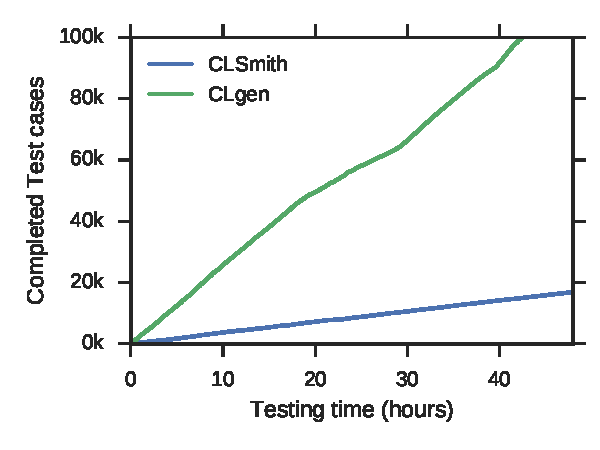
\includegraphics[width=\columnwidth]{build/img/total-tests}%
%	\caption{%
%		Test cases. \cc{TODO: Replot with the fastest and slowest device for each}%
%	}%
%	\label{fig:total-tests} %
%\end{figure}
